% Notes: 
% Here we describe how the work was done.
% Mathematical description of new model. Maybe pseudocode of algorithm? 
% Discussion of new model? Performance, complexicity, etc? 
% We describe the extended isolation forest here. In Direct Analysis of GD .. the used method has its own section. 
% Concept, and new stuffs
% Running isolation as is directly on bases - phase 1
% Running extended isolation on the bases  - phase 2
% Can include or exclude counts 
% tradeoffs: counts, precision. 

% -----------

% What to include:

\subsection{Isolation Forest on GD compressed Data}
Data compressed with generalized deduplication results in having a set of bases, deviation and references linking a data point to its base and deviation. In the following example the deviation will be omitted. Say we have the data set $S$ where $S \in \mathbb{R}^2$. Performing GD on $S$ will result in each feature of the points being mapped to their bases. Having an point $x = [x_1,x_2]$ where $x \in S$ and some computed bases ids $b_0, b_1, ..., b_n$,then the transformed version $x*=[x^*_1, x^*_2]$ will hold the computed bases. This is depicted on Figure \ref*{fig:gd_points}. The bases are computed on the raw data and referenced in the features $x^*_1$ and $x^*_2$.

\begin{figure}
  \centering
  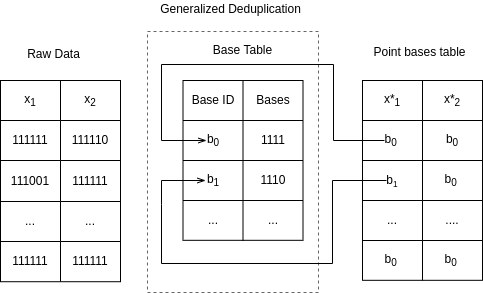
\includegraphics[width=\linewidth]{../files/test.png}
  \caption{}
  \label{fig:gd_points}
\end{figure}

Isolation forest is then to be performed on the transformed version of the data set. The isolation forest splits before compression could be seen on Figure \ref{fig:rich_sketch_original}. Figure \ref{fig:rich_sketch_bases} is similar but is instead performing the splits on the bases. It is seen that certain data points will map to identical bases on both features.  

\begin{figure}
  \centering
  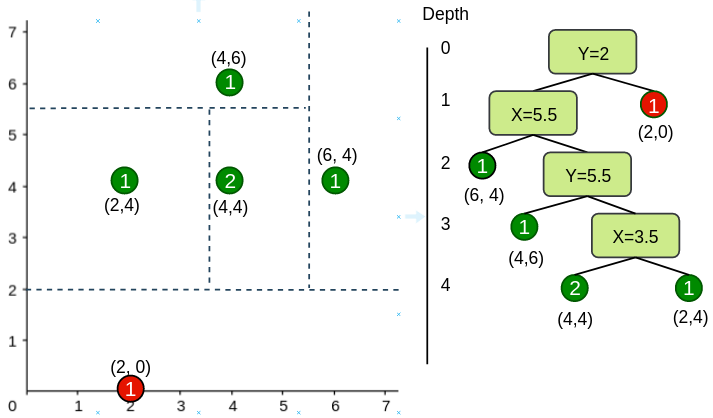
\includegraphics[width=\linewidth]{images/rich_sketch_bases.png}
  \caption{}
  \label{fig:rich_sketch_bases}
\end{figure}


\subsection{DupRes Isolation Forest}
The bases of GD compressed data will inherintly be grouped. Stripping the deviation of each data point will result in data points being placed in bins. This binning is illustrated on Figure \ref{fig:binning-1} and \ref{fig:binning-2}. The graphics shows the bins created with different amount of deviation bits. The circles are samples. The dotted lines are enclosing areas where data points in an area will be mapped to the closest base in the negative direction. The arrows illustrate the base each data point will be mapped to. Having a larger amount of deviation bits is leading to larger bins. 

\begin{figure}
  \centering
  \begin{minipage}{0.45\linewidth}
      \centering
      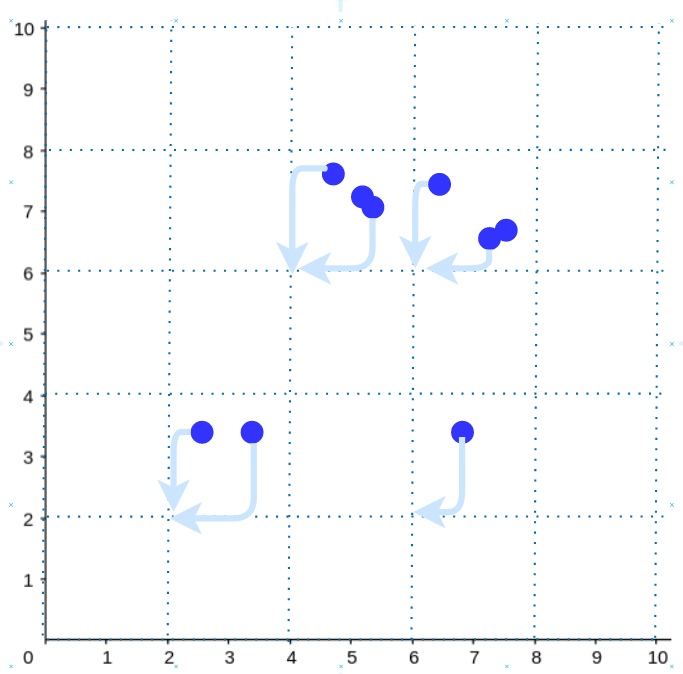
\includegraphics[width=\textwidth]{images/binning-1dev.png}
      \caption{first figure}
      \label{fig:binning-1}
  \end{minipage}\hfill
  \begin{minipage}{0.45\linewidth}
      \centering
      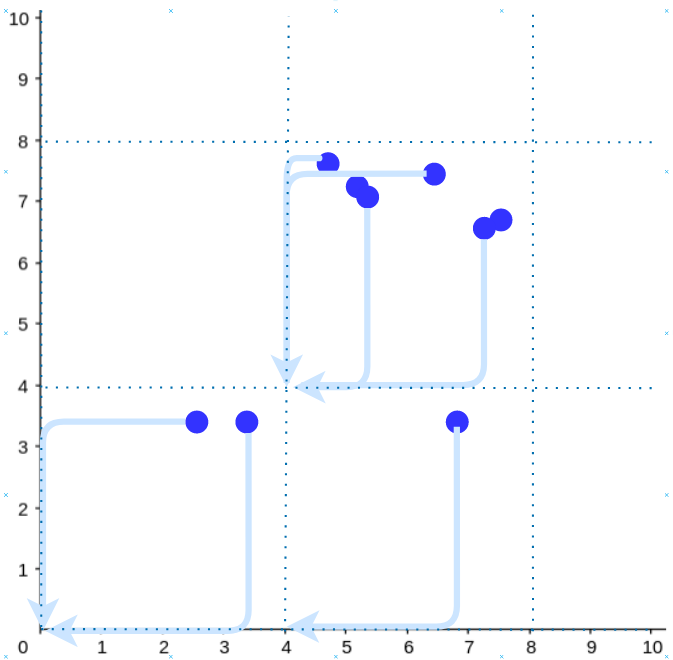
\includegraphics[width=\textwidth]{images/binning-2dev.png}
      \caption{first figure}
      \label{fig:binning-2}
  \end{minipage}
\end{figure}

Having larger bins might lead to a better compression rate however it could lead to undesired behaviour when trying to detect anomalies with iForest. An outlier could be mapped to the same base as an inlier on all or some of it features. Having the same base on some features will make it harder to isolate the outlier meanwhile having identical bases on all features makes it impossible. The binning aswell leads to inliers being grouped on fewer points. This causes them to be isolated more easily, and thus labeled as outliers.   

Isolation Forest is not fit for the large amount duplicates that is potentially created by compressing with generalized deduplication. Therefore, a more duplicate resistant (DupRes) version is proposed. The core idea of the new version is to utilize the amount of duplicates when building the tree. The amount is then used to adjust the score of an observation. A revised version of the score function is: 

\begin{equation}
  s(x,n) = 2^{-\frac{E(h(x))+log_2(x_{count})}{c(n)}}
  \label{eq:dupres_score}
\end{equation}     
 
The new function differs from Equation \ref{eq:org_score} by the introduction of the $log_2(x_{count})$ term. $x_{count}$ is the amount of occurences of the given sample. The reason behind using the binary logarithm is firstly that having one occurance will not modify the score, $log_2(1)=0$. Secondly, it is a strictly increasing function. Resulting in the higher the $x_{count}$, the larger adjustments will be made to the score. The modification makes no changes in the range of $s$ and in how it should be interpreted. For further details, see the original paper \cite{iforest}.     

The change implies that the count of each sample is known. This requires extending what is done in the training phase of the model. Beside building the decision trees, the model must store each unique sample with the amount of occurences. Worst case the training set contains no duplicates and will store all training samples with the count of one. Hereby, the model is not optimal if the data is expected to have a low amount of duplicates. The flow during the evaluation of unseen observations, is to identify the ones that was seen in the training phase and retrive their counts. The adjusted score is then computed and can be used to identify anomalies.        

% amount features 
% figure with grouped 
% What is the new method, formulas, tweak log thingy. Training, testing.. 
% - storing all train data in memory :( 
% - how did we derive equations. One more for prins knud. 
% 
